\chapter{Rendering of Implicit Surfaces}\label{s:rendering-of-implicit-surfaces}
We've known what a implicit surface is and how to represent it. Now we are going to discuss how to render a implicit surface. 

But before getting into it, let's talk about different representation and it's rendering techniques. Because comparing two different solutions, which actually solve the same problems, always makes us understand both better. In this section, we will first talk something about rasterization and raytracing; next we will introduce the general raytracing technique for volume representation and it' improved version, sphere tracing, for distance fields representation; Lastly, we will discuss some enhancement of sphere tracing method. 


\section{Representation and Rendering}
There are two main ways to draw 3D: rasterization and ray tracing. They use different method to represent a scene and to render it. As aforementioned in the parametric surfaces section, a parametric surface defines every point in $R^{n-1}$ domain, we usually use a mesh which consist of many triangles, all vertexes of which discretized the surface, to represent it in a scene. In the rendering time, CPU will send the mesh data, which contains vertexes, indexes and normals etc, to GPU and the GPU will raster the vertexes to provide the position of a single point to the shaders, which use it to shader the pixel. Usually, a Gouraud shading, which computing the lighting at the corners of each triangle and linearly interpolating the resulting colours for each pixel covered by the triangle, or Phong shading, which interpolates surface normals across rasterized polygons and computes pixel colors based on the interpolated normals and a reflection model, is used. For a long time these two techniques remained the two main means of lighting 3D imagery objects. Even in today, we still use this methods but add some physically effects.

This method, by using meshes represent surface and using GPU to rasterize it, we call it $rasterization$, has some advantage: Graphics hardware is optimized to support it and it's fast. But it also has more seriously problems: it can not support indirect illumination and it's performance approximately linear to number of triangles and lights. Some techniques have been introduced to it, such as indirect lighting cache, environment maps, shadow maps etc, to make the rendered images more realistic. But these techniques rely on precomputation, which can not be used for dynamic scenes. We need another ways which can simulate the real world's phenomenon more naturely.  

\begin{figure}
\sidecaption
	\includegraphics[width=.65\textwidth]{graphics/df/Ray_trace_diagram}
	\caption{The ray tracing algorithm builds an image by extending rays into a scene(Images from Henrik).}
	\label{f:ray-tracing-diagram}
\end{figure}
	
The most important technique which can achieve this goal is \textit{ray tracing}. The first ray tracing algorithms cast rays from the eye into scene until they hit an object, but the rays were not traced any further. The next important research breakthrough came from Turner Whitted\cite{a:ray-tracing}.  

In Whitted's way, when a ray hits a surface, it can generate up to three new types of rays: reflection, refraction, and shadow. A reflection ray is traced in the mirror-reflection direction. The closest object it intersects is what will be seen in the reflection. Refraction rays traveling through transparent material work similarly, with the addition that a refractive ray could be entering or exiting a material. A shadow ray is traced toward each light. If any opaque object is found between the surface and the light, the surface is in shadow and the light does not illuminate it. This recursive ray tracing added more realism to ray traced images.

\begin{figure*}
	\begin{subfigure}[b]{0.5\textwidth}
		\includegraphics[width=1.0\textwidth]{graphics/df/explaination-brdf2}
		\caption{from incoming(light) direction.}
	\end{subfigure}
	\begin{subfigure}[b]{0.5\textwidth}
		\includegraphics[width=1.0\textwidth]{graphics/df/explaination-brdf1}
		\caption{from outgoing(view) direction.}
	\end{subfigure}
	\caption{a: for a given incoming light, some will be reflected in a small directions(specular) and some will be scattered to all directions(diffuse). b is an alternative interpretation - that a outgoing light comes from many incoming lights.(Images from Real-Time Rendering, 3rd edition).}
	\label{f:brdf}
\end{figure*}

At a point of a surface, the outgoing light could come from many directions, see figure \ref{f:brdf}. So at every point for ray tracing, we should cast multi-rays to compute reflection, refraction, and shadow. For a good result, every point may needs hundreds of new rays, recursively, the hundreds of rays need another thousands of new rays. For a single frame, a scene may needs billions of rays, That's a huge cost even for the offline films. But it can generate the most realistic images, see figure \ref{f:ray-tracing-result}. 

So for ray tracing, it usually use \textit{Monte Carlo algorithms} to solve the integral problems.   

In ray tracing, the most hard part is ray-surface intersection calculation. In a explicit surface representation, for every intersection, we must check every triangle of every object in the scene. For acceleration, some partitioning techniques, such as Octree, kdtree etc , have been introduced. Even so, it still costly in an interactive environment.

\begin{figure}
\sidecaption
	\includegraphics[width=.65\textwidth]{graphics/df/Voxelgitter}
	\caption{Illustration of a voxel grid, each containing a color value(Images from wikipedia).}
	\label{f:volume-representation}
\end{figure}

For avoiding ray-surface intersection calculation, one way is to define every point of the scene. This leads to \textit{voxel representation}, see figure \ref{f:volume-representation}, a object is discretized to voxel grid. Then a ray can check intersection directly, no needs to iterative every object. The voxels between the discrete grids can be interpolated using bilinear or other filter which supported by GPU. The process of voxelize a object is called \textit{voxelization}.

\begin{figure}
	\includegraphics[width=1.0\textwidth]{graphics/df/ray-tracing-result}
	\caption{Ray tracing can create realistic images(Images from Gilles Tran).}
	\label{f:ray-tracing-result}
\end{figure}

In a voxel representation, a usually used technique is ray marching, which we will discuss in the next section. Voxel model usually represent explicit surfaces, the value of a single voxel is a color. 

Sine implicit surface, like distance field, can be represent as volume texture, we could use ray tracing easily. Even more, in a distance filed, every grid is a distance (not a color), we can use a more efficiently way, which is called \textit{sphere tracing}, will be introduced follows.    

And the introduction of ray tracing make us have chance to get some global illumination effect, that's what we need. In this article, we will discuss some these kind of applications.




\section{Ray Marching}
Traditionally, objects are modelled as sets having infinitesimally thin boundary surfaces. Often a computed or digitized texture or displacement is then mapped onto the surface for enhanced realism. 

\begin{figure}
	\begin{subfigure}[b]{.32\textwidth}
		\includegraphics[width=1.0\textwidth]{graphics/df/hypertexture1}
	\end{subfigure}
	\begin{subfigure}[b]{.32\textwidth}
		\includegraphics[width=1.0\textwidth]{graphics/df/hypertexture2}
	\end{subfigure}
	\begin{subfigure}[b]{.32\textwidth}
		\includegraphics[width=1.0\textwidth]{graphics/df/hypertexture3}
	\end{subfigure}
	\caption{Some images are made with hypertexture(Images courtesy of Perlin).}
	\label{f:hypertexture}
\end{figure}

However, many objects, such as fur or woven materials, have a complex definition which is at best awkward, and at worst impossible, to describe by a surface model. For other objects, such as eroded materials or fluids, a highly complex boundary is actually an artifact of a process that is often more readily described volumetrically. Still other objects, such as flame, clouds, or smoke, don't actually have a well defined boundary surface at all.

Ken Perlin has found in \cite[5mm]{a:hypetrtexture}, that the appearance of many such objects can be described directly by some applicative function, evaluated over a sampling of some region of $R_{3}$. They use a called \textit{Hypertexture} (see figure \ref{f:hypertexture}) to define an intermediate region between object and non-object, which has the following concepts:

\begin{itemize}
	\item an \textit{Object Density Function $D(x)$} with range [0,1] which describes the density of a 3D shape for all points $x$ throughout $R_{3}$. The \textit{soft region} of an object consists of all $x$ such that $0<D(x)<1$. 
	\item a \textit{Density Modulation Function (DMF)} $f_{i}$, which is used to modulate an object's density within its soft region. Each DMF is used to control some aspect of an objects' spatial characteristics; a collection of DMF's comprises a volume modelling toolkit.   
\end{itemize}

Hyper texture is created by successive application of DMFs $f_{i}$ to an object's $D(x)$:

\begin{equation}
	H(D(x),x)=f_{n}(...f_{2}(f_{0}(D(x))))
\end{equation}

Formally, a soft object is a density function $D(x)$ over $R_{3}$, where  $D$ is 1.0 inside the object, 0.0 outside the object, and $0.0<D<1.0$ in a region of nonzero thickness in between.

Since hypertexture is a volume representation in $R_{3}$, and it often has no well defined surfaces, it is only practical using volume rendering techniques. They use ray marching algorithm.

In traditional ray casting, the ray marcher casts a ray into model space for every pixel. But they first clip each ray to a parallelpiped that bounds the hypertexture volume. If the ray does not intersect the parallepiped, they move to the next pixel for processing. If the ray dose intersect the parallepiped, the ray parameters $\mu_{0}$ and $\mu_{1}$, representing respectively the entry and exit points of the parallelpiped, are computed. Ray marching begins at ray parameter value $\mu_{0}$, and proceeds at a fixed increment $\Delta\mu$. Sampling the model along the ray at points:

\begin{figure}
\sidecaption
	\includegraphics[width=.65\textwidth]{graphics/df/ray-marching}
	\caption{Ray marching has a constant steps.}
\end{figure}

\begin{equation}
	x=x_{\mu_{0}}+k\Delta x_{\mu}
\end{equation} 

where $k=0,1,2,...$ such that $\mu_{0}+k\Delta\mu\leq\mu_{1}$, and $\Delta x_{\mu}$ is the displacement along the ray, in model space at each increment.


Here is the pseudo code of ray marching:

\begin{algorithm}
\begin{lstlisting}[mathescape]
$k=0$
$d=0$
while $k < k_{max}$ do
	d = f(r(k))
	if $d\leq 0$ then return $k\Delta t$
	$k=k+1$
	return 0
\end{lstlisting}
\caption{Ray marching pseudo code}
\end{algorithm}
   

\begin{figure}\label{f:ray-marching-problems}
	\begin{center}	
		\includegraphics[width=1.\textwidth]{graphics/df/ray-marching-problems}
	\end{center}
	\caption{Ray marching. Surface represented by the blue contour, green dots are sampling points along the ray whose spacing is determined by the step size.}
\end{figure}

It should be noted that ray marching has some problems, see figure \ref{f:ray-marching-problems}. If the steps are too large one can traverse too far into the interior of the surface and therefore loose accuracy of the overall surface shape. Moreover, it is even possible to miss the surface completely or some parts of it. So the distance that the ray travels between steps should be as small as possible in order to better estimate the boundary region of the surface.


We will see, this problems can be solved by using distance field representation. And this is the difference between ray marching and sphere tracing; it's also the difference between general voxel representation (which may base on explicit surface or procedure functions) and implicit surface representation.

\section{Sphere Tracing}
By using distance field representation, the value of a voxel is not a color, it's a distance to the closet surface, which means that we can not render it directly. We must (or could) use it, this distance value, to find the point, which is the ray-surface intersection, on the surface along the ray. This is the difference between ray marching and sphere tracing, although they look similar. 

\begin{figure}
	\includegraphics[width=1.0\textwidth]{graphics/df/sphere_tracing}
	\label{f:sphere-tracing}
	\caption{In sphere tracing, the step is dynamically decided by the distance value, and it keeping marching until it reach to the maximal distance or hit a surface.}
\end{figure}

At a point of a distance filed,  if we draw a sphere around it's self and use it's distance value as the radius. Then it could guarantee that there is no objects in the sphere, which is called \textit{unbounding volumes} in \cite{a:Ray-Tracing-Deterministic-3-DFractals}. Hence, we could use this radius as the step of the ray marching, which has a variant steps. If we keep marching by this way along the ray, we can finally find the point on some surface which intersect with the ray.The process can be figure out from figure \ref{f:sphere-tracing}. That's why we call it \textit{sphere tracing}.

To end it, we both use a maximal distance $D$ the ray can traverse and a minimal distance $\varepsilon$, which is usually a very small number, denotes the desired precision of the convergence test. The pseudo code as showing in algorithm \ref{lst:sphere-tracing]}.


By using the implicit surface representation, which provides a faster ray tracing computing. We could use this power to do some degree of global illumination effect. Even we can not replace the traditional rasterization right now, but we can replace some static precomputation, which make our game more dynamically. 

\begin{algorithm}\label{lst:sphere-tracing]}
\begin{lstlisting}[mathescape]
$k=0$
$d=0$
while $t < D$ do
	d = f(r(t))
	if $d\leq\varepsilon$ then return $t$
	$t=t+d$
	return 0
\end{lstlisting}
\caption{Sphere tracing pseudo code.}
\end{algorithm}

The most important, we are getting closer to ray tracing!

\section{Enhanced Sphere Tracing}
It should be fast, if the whole scene is a single volume texture, every step is just a sampling operation, which get the next march distance, and a comparing operation, just like the pseudo code \ref{lst:sphere-tracing}. 

But we have been told that for saving memory we should use a hierarchy like structure, such as ADFs use Octree represent the scene. In these hierarchy ways, usually only a single object is a small, low resolution volume texture, and the whole picture combines all the objects as a hierarchy distance field, see figure \ref{f:visualize-mesh-distance-fields}.

\begin{figure}\label{f:visualize-mesh-distance-fields}
	\includegraphics[width=1.0\textwidth]{graphics/df/VisualizeMeshDistanceFields}
	\caption{A visualization of the mesh distance fields in a level in Unreal Engine 4. Every mesh instance can generate a distance field, and the whole scene is represented by some hierarchy structure(Images courtesy of Unreal Engine 4 Documentation). }
\end{figure}

This makes the performance matter. In this section we will introduce some enhancement of sphere tracing, mainly global distance and over-relaxation sphere tracing. The basic idea is reduce the marching times. 

\subsection{Far from the Surface}
The the current point of a ray is far from the surface, or when it is in a large empty space, it should has a big step. 

Since the distance field usually only represent objects not empty space, some uses bounding box (or sphere) marks the empty spaces. The interesting method is come from Unreal Engine 4, beside generating a single distance field for every mesh object, they also use all of the per-object distance fields to generate a global distance field. 

\begin{figure}\label{f:global-distance-field}
	\includegraphics[width=1.0\textwidth]{graphics/df/DF_GlobalDF}
	\caption{On the right are all per-object distance fields, only the objects in the scene have been computed; On the left is the global distance field, the ray can across the large empty space easily(Images from Unreal Engine 4 Documentation).}
\end{figure}

The global distance field is lower resolution than the object distance fields. They use it when computing cone traces for sky occlusion, the object distance fields are sampled near the point being shaded, while the much faster global distance field is sampled further away. see figure \ref{f:global-distance-field}.

\subsection{Over-relaxation Sphere Tracing}
In iterative methods, the \textit{successive overrelaxation method (SOR)}\footnote{\url{https://en.wikipedia.org/wiki/Successive_over-relaxation}} is a method of solving a linear system of equation $Ax=b$ derived by extrapolating the Gauss-Seidel method. This extrapolation takes the form of a weighted average between the previous iterative and the computed Gauss-Seidel iterative successively for each component:

\begin{equation}
	x_{i}^{(k)}=\omega\vec{x}_{i}^{(k)}+(1-\omega)x_{i}^{(k-1)}
\end{equation}

where $\vec{x}$ denotes a Gauss-Seidel iterate and $\omega$ is the extroplation factor. The idea is to choose a value for $\omega$ that will accelerate the rate of convergence of the iterative to the solution. If $\omega=1$, the SOR method simplifies to the Guass-Seidel method. A theorem due to Kahan (1958) shows that SOR fails to converge if $\omega$ is outside the interval (0,2).

Another enhancement of sphere tracing comes from \cite{a:Enhanced-Sphere-Tracing}, which apply the principle of over-relaxation to sphere tracing: Instead of stepping along the ray using the radius of the unbounding sphere at each iterative, a step size $\delta_{i}=f(p_{i})\cdot\omega$ can be used, where $f(p_{i})$ denotes the value of the signed distance bound at the position of $i-$th iteration and $\omega\in[1;2)$ the relaxation parameter.

\begin{figure}\label{f:over-relaxation}
	\includegraphics[width=1.0\textwidth]{graphics/df/over-relaxation}
	\caption{Comparison of sphere tracing without (top) and with over-relaxation method (bottom). Blue circles denote iteration steps conducted with standard sphere tracing, red circles denote steps with over-relaxation using $\omega=1.6$. The rightmost red circle and the yellow circle show an iteration step where over-relaxation fails (i.e. the circles do not overlap). The arrow points towards $p_{fallback}$ which is used as a starting point for completing tracing of the ray after over-relaxation failure has been detected.}
\end{figure} 

They treat every step of ray marching as one iterative. Because over-relaxation guarantee the result will converge to the correct result, so if ahead of the ray is empty space, using over-relaxation will makes the marching more quickly. But if there is a small sphere, then we are not applying iterative method any more, we should fallback to a normal step:

\begin{equation}
	p_{fallback}=p_{i}+d\cdot\delta_{i-1}\cdot(1-\omega)
\end{equation}

We can see, actually this is not a real application of SOR, we are not guessing and there is not a $Ax=b$ equation. We only use the concept that if there are empty space, we can treat the current $f(p_{i})$ as the equation, but we are still not guessing. Or you can think that if there is a cone which origin at the ray's origin, and at point $p_{i}$ the radius is $f{p_{i}}$, then then marching step, $f(p_{i})\cdot\omega$, guarantee that the marching will never touch the out side of cone but with a faster speed.
 

 
\subsection{Optimization for Convex Objects}
Also in the same paper, another technique has been introduced to accelerate the tracing of convex object, see figure \ref{f:convex-objects}.

\begin{figure*}\label{f:convex-objects}
	\includegraphics[width=1.0\textwidth]{graphics/df/Optimization-for-Convex-Objects}
	\caption{Illustration of optimization for sphere tracing through convex objects represented by a signed distance bound. From left to right: Convex object enclosed by a convex bounding volume; ray origin inside bounding volume but outside the object; ray origin outside bounding volume and outside the object; ray origin inside the object and bounding volume with sphere tracing from the outside; the same scenario as the previous with sphere tracing through the interior of the object.}
\end{figure*}

We've known that usually every object has it's own distance field, and most of the objects are polygon. If the object is convex object, it can reduce the times of marching when the ray pass though it. The paper considers three cases:

\begin{enumerate}
	\item Ray origin outside bounding volume
	\item Ray origin inside bounding volume and outside the object
	\item Ray origin inside bounding volume and inside object
\end{enumerate} 

In case 1, it keeps the marching as usual, there is no need to change; In case 2, no matter how a ray enter the distance field of the object, it origins from the intersection with the boundary geometry, which compute a big step to the surface; In the case 3, if a ray origins from inside of the object, which first find the intersection of the ray with the bounding geometry, then they perform sphere tracing in the inverse ray direction, starting at the intersection with the bounding object, which yields the same intersection point as if having traced through the object. In case 4, if the marching is costly, such as it will beyond the maximum distance, it will be avoided completely. 

\begin{figure}
\begin{center}
	\includegraphics[width=0.85\textwidth]{graphics/df/enhanced-sphere-tracing}	
\end{center}
	\caption{Enhanced sphere tracing uses consecutive bounds to increase ray march throughput by 25\%-100\%.}
\end{figure} 

This paper is also contain other methods can enhance the sphere tracing, which mainly can improve the visual quality and reduce artifacts. The following real-time scene is rendered by these enhanced techniques.


 \begin{figure}
 	\includegraphics[width=1.0\textwidth]{graphics/df/enhanced-sphere-tracing-result}
 	\caption{Comparison of the number of iterations required without over-relaxation (left) and with (w = 1.2) (right). The image shows the number of iterations at which a ray terminates. Note, how more buildings become visible in the distance in the right image since the maximum number of iterations (80) is reached less quickly.}
 \end{figure}









\chapter{Rendering of Glyphs}
Now we are going to discuss lots of applications of distance field. That's so exciting because I've never seen an simple concept, you can use few words tell someone what DF is, can solve so many problems. furthermore, these applications cover lots of different areas, And there should and would be more.

These applications are not focus on rendering a distance field represented surface, but mostly use it as a tool to assist other problem computation. Because rendering implicit surface on real time is still costly, hight quality result requires high resolution volume textures or more complex representation data structure. So that's the reason the volume's resolution in these applications is low and that guarantees the performance. 

Low resolution DF, That's where we will start from.

The first thing I got know about distance field is Chris Green's paper \cite{a:improved-alpha-tested-magnification-for-vector-txtures}, which provided an improved alpha-tested magnification for vector and special effects. This method has been mainly used to render glyphs in game industry.  

\begin{figure}\label{f:magnification}
	\begin{subfigure}[t]{0.298\textwidth}
		\includegraphics[width=1.0\textwidth]{graphics/df/magnification}
		\caption{simple bilinear filtering}
	\end{subfigure}
	\begin{subfigure}[t]{.33\textwidth}
		\includegraphics[width=1.0\textwidth]{graphics/df/alpha-testing}
		\caption{alpha testing}
	\end{subfigure}
	\begin{subfigure}[t]{.33\textwidth}
		\includegraphics[width=1.0\textwidth]{graphics/df/distance-field-glyph}
		\caption{distance field technique}
	\end{subfigure}
	\caption{Vector art encoded in a $64x64$ texture.}
\end{figure}

Textures are magnified in GPU will generate "jaggies", Although the hardware bilinear filtering will make it looks smooth, but it also make the image looks blurry, see figure \ref{f:magnification}(a). 


If this is a bitmap, hardware filtering is the only choice we have, other wise it requires a very high resolution texture to avoid being magnified (but which can not be avoided forever, the camera always could move closer). But if it is a vector "line-art" images, all the matter thing is the ability to distinguish the border, and the inside will be rendered by some other non-texture-mapping technique, then we could use alpha testing. See figure \ref{f:magnification}(b), a glyph's color is a uniform parameter of the shader, not sampling from the texture, and we only use alpha-testing technique to find the border. This gives us a very clear images.

But the alpha value is still sampled from the texture, so the alpha value itself is jaggied. And there is no way we can totally avoid sampling. This leads us to find a way which could narrow a wide blurred band to a thin clear strip. This method should generate the result like figure \ref{f:magnification}(c). 

There is that kink of method which called \textit{smoothstep}\footnote{\url{https://en.wikipedia.org/wiki/Smoothstep}}, and which has been provided by GPU hardware.

Smoothstep is a scalar function which interpolates smoothly between two input values based on a third one that should be betwenn the first two. The return value is clamped between 0 and 1:

\begin{equation}
	smoothsetp(min,max,x)=
	\begin{cases}
		0,& \text{if } x\leq min\\
		(0,1) &\text{if } x\in(min,max)\\
		1,& \text{if } x\geq max
	\end{cases}
\end{equation} 

The slop of the smoothstep (see figure \ref{f:smoothstep}) function tends toward zero at both edges, and the input $x$ get more close to the center of $[min,max]$, it's output get to $0.5$ quicker. This will makes a range $[min,max]$ more narrow in the middle of the range. smoothstep pluses a threshold will make the border smoother.

A example provided by DirectX and OpenGL is:

\begin{equation}
	smoothstep(t)=3t^{2}-st^{3}
\end{equation}

And a more smoother version is:

\begin{equation}
	smootherstep(t)=6t^{5}-15t^{4}+10t^{3}
\end{equation}

That's cool, but our texture is a alpha image, 0 means outside and 1 means inside. The border representation is not a range. That make us think the represent the border as a range, and this idea is absolutely the same as distance field.

\begin{figure}\label{f:smoothstep}
	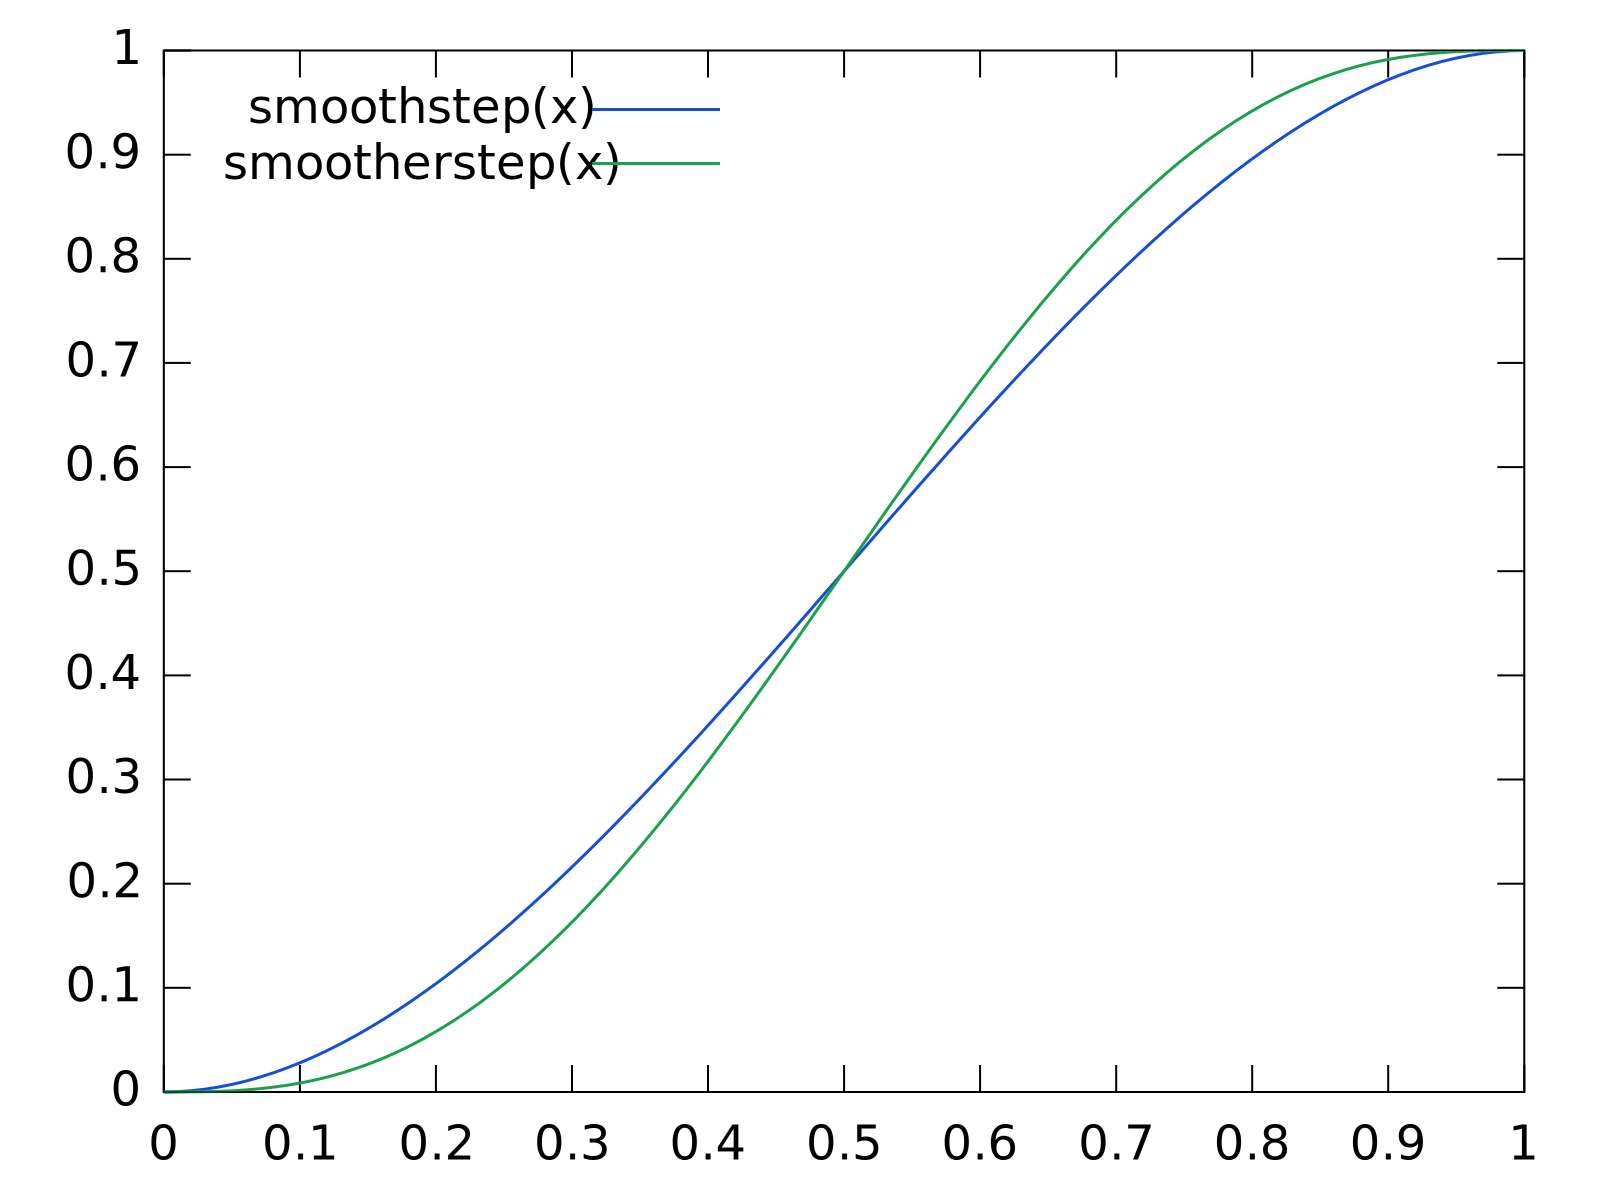
\includegraphics[width=1.0\textwidth]{graphics/df/Smoothstep_and_Smootherstep}
	\caption{A plot of the smoothstep(x) and smootherstep(x) functions(Images from wikipedia).}
\end{figure}

The chose to generate the low-resolution distance field from high resolution source image. In a typical case, a 4096x4096 image will be used to generate a distance field texture with a resolution as low as 64x64, as shown in figure \ref{f:glyph-distance-field}. And the distance field represented texture is stored in an 8-bit channel. In rendering time, the distance value is first sampled from texture using the bilinear texture interpolation which is present in all modern GPUs in order accurately reconstruct the distance between a sub-texel and a picewise-linear approximation of the true high-resolution image. 

\begin{figure}
	\begin{subfigure}[t]{.48\textwidth}
		\includegraphics[width=1.0\textwidth]{graphics/df/high-resolution-glyph}
		\caption{Hight resolution input}
	\end{subfigure}
	\begin{subfigure}[t]{.48\textwidth}
		\includegraphics[width=1.0\textwidth]{graphics/df/distance-field-of-glyph}
		\caption{64x64 Distance field}
	\end{subfigure}
	\caption{(a) A high resolution (4096x4096) binary input is used to compute (b) a low resolution (64x64) distance field.}
	\label{f:glyph-distance-field}
\end{figure}


The paper also provided some other effects about outlining, glows, shadows and sharp corners. But almost all of them use the basic ideas we just discussed. I'm sure you will understand them well.

About this application, we should get from that, sometimes, there is no need to store a high resolution distance field volume. This basic idea would and should keep in mind when reading the next applications.   


